\section{The Zigbee Protocol}
\label{background}
Zigbee is a low-cost, low-power wireless communication protocol designed for short-range communications, making it well suited for embedded systems and smart home applications. Its support for mesh networking enables the deployment of robust and self-healing networks with extended coverage. Zigbee is built on top of the IEEE 802.15.4 standard \cite{ieee_802_15_4}, which specifies low-rate wireless personal area networks (LR-WPANs) optimized for low data rates and minimal energy consumption.

\subsection{Zigbee Network Architecture}
The Zigbee protocol stack consists of four layers: the physical (PHY) layer, the medium access control (MAC) layer, the network (NWK) layer, and the application (APL) layer. The PHY and MAC layers are defined by IEEE 802.15.4 and are responsible for physical transmission and channel access control.

IEEE 802.15.4 operates over multiple frequency bands to accommodate regional regulations. In the widely adopted 2.4~GHz band, it supports 16 channels with 5~MHz spacing. The MAC layer employs a contention-based access mechanism based on CSMA/CA. In beacon-enabled networks, the PAN Coordinator periodically transmits beacon frames containing network parameters and synchronization information.

Building on IEEE 802.15.4, Zigbee introduces the NWK and APL layers to enable multi-hop routing, network management, and application-level services. The application layer includes the Application Support Sublayer (APS), the Zigbee Device Object (ZDO), and an application framework defining device-specific operations. The APS handles data binding, fragmentation, and security, while the ZDO is responsible for network formation, device discovery, and security configuration. Although Zigbee application profiles promote interoperability, their standardized data formats can increase the complexity of traffic-based device classification.

Zigbee networks comprise three main device roles: the \gls*{panc}, Full Function Devices (FFDs), and Reduced Function Devices (RFDs). The \gls*{panc} manages network creation, addressing, and coordination. FFDs, commonly acting as routers, relay packets on behalf of other devices and enable multi-hop communication, which allows Zigbee networks to extend coverage without relying on a high-power central access point. RFDs are typically low-power sensors or actuators that communicate through routers or directly with the \gls*{panc}.

Each Zigbee device is uniquely identified by a 64-bit IEEE MAC address (extended address). After joining the network, a 16-bit short address is assigned by the coordinator and used for subsequent intra-network communications.

These architectural characteristics have direct implications for traffic observability and analysis, particularly in forensic scenarios involving multi-hop communications and dynamically evolving network topologies.

%\begin{figure}[]
%    \centering
%    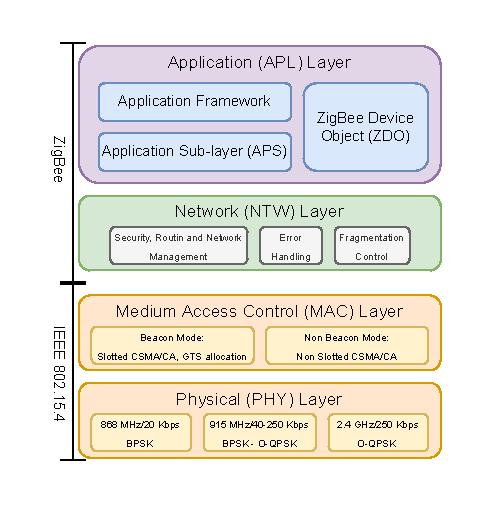
\includegraphics[width=\linewidth]{Figures/zigbeestack.drawio.pdf}
%    \caption{IEEE 802.15.4 and ZigBee protocol stack architecture}
%    \label{zb_stack}
%\end{figure}
